\appendix

\clearpage
\section*{Appendix}
\addcontentsline{toc}{section}{Appendix}

\section{Previous EWS FEM work}
\label{sec:appendix_previous_ews_fem_work}

The present project was developed in the context of previous internal Early Warning Scan (EWS) finite element modelling work. Earlier EWS models provided a methodological starting point for parametrised breast geometry, soft-tissue material assumptions, dynamic loading and displacement-based evaluation \cite{EngelsEWSReport, StormEWSReport}. These previous projects were used as internal engineering reference material and as a comparison point for modelling choices. They were not used as validation datasets for the current COMSOL model.

The earlier FEBio-oriented modelling route used a simplified parametrised breast representation in which adipose and glandular regions were defined from geometric construction parameters. Figure~\ref{fig:appendix_previous_ews_cross_section} shows a schematic cross-section from the earlier EWS project by R. Engels \cite{EngelsEWSReport}. This representation provided useful context for the transition toward a COMSOL-based workflow, but the current COMSOL model does not reproduce the previous geometry directly.

\begin{figure}[H]
\centering
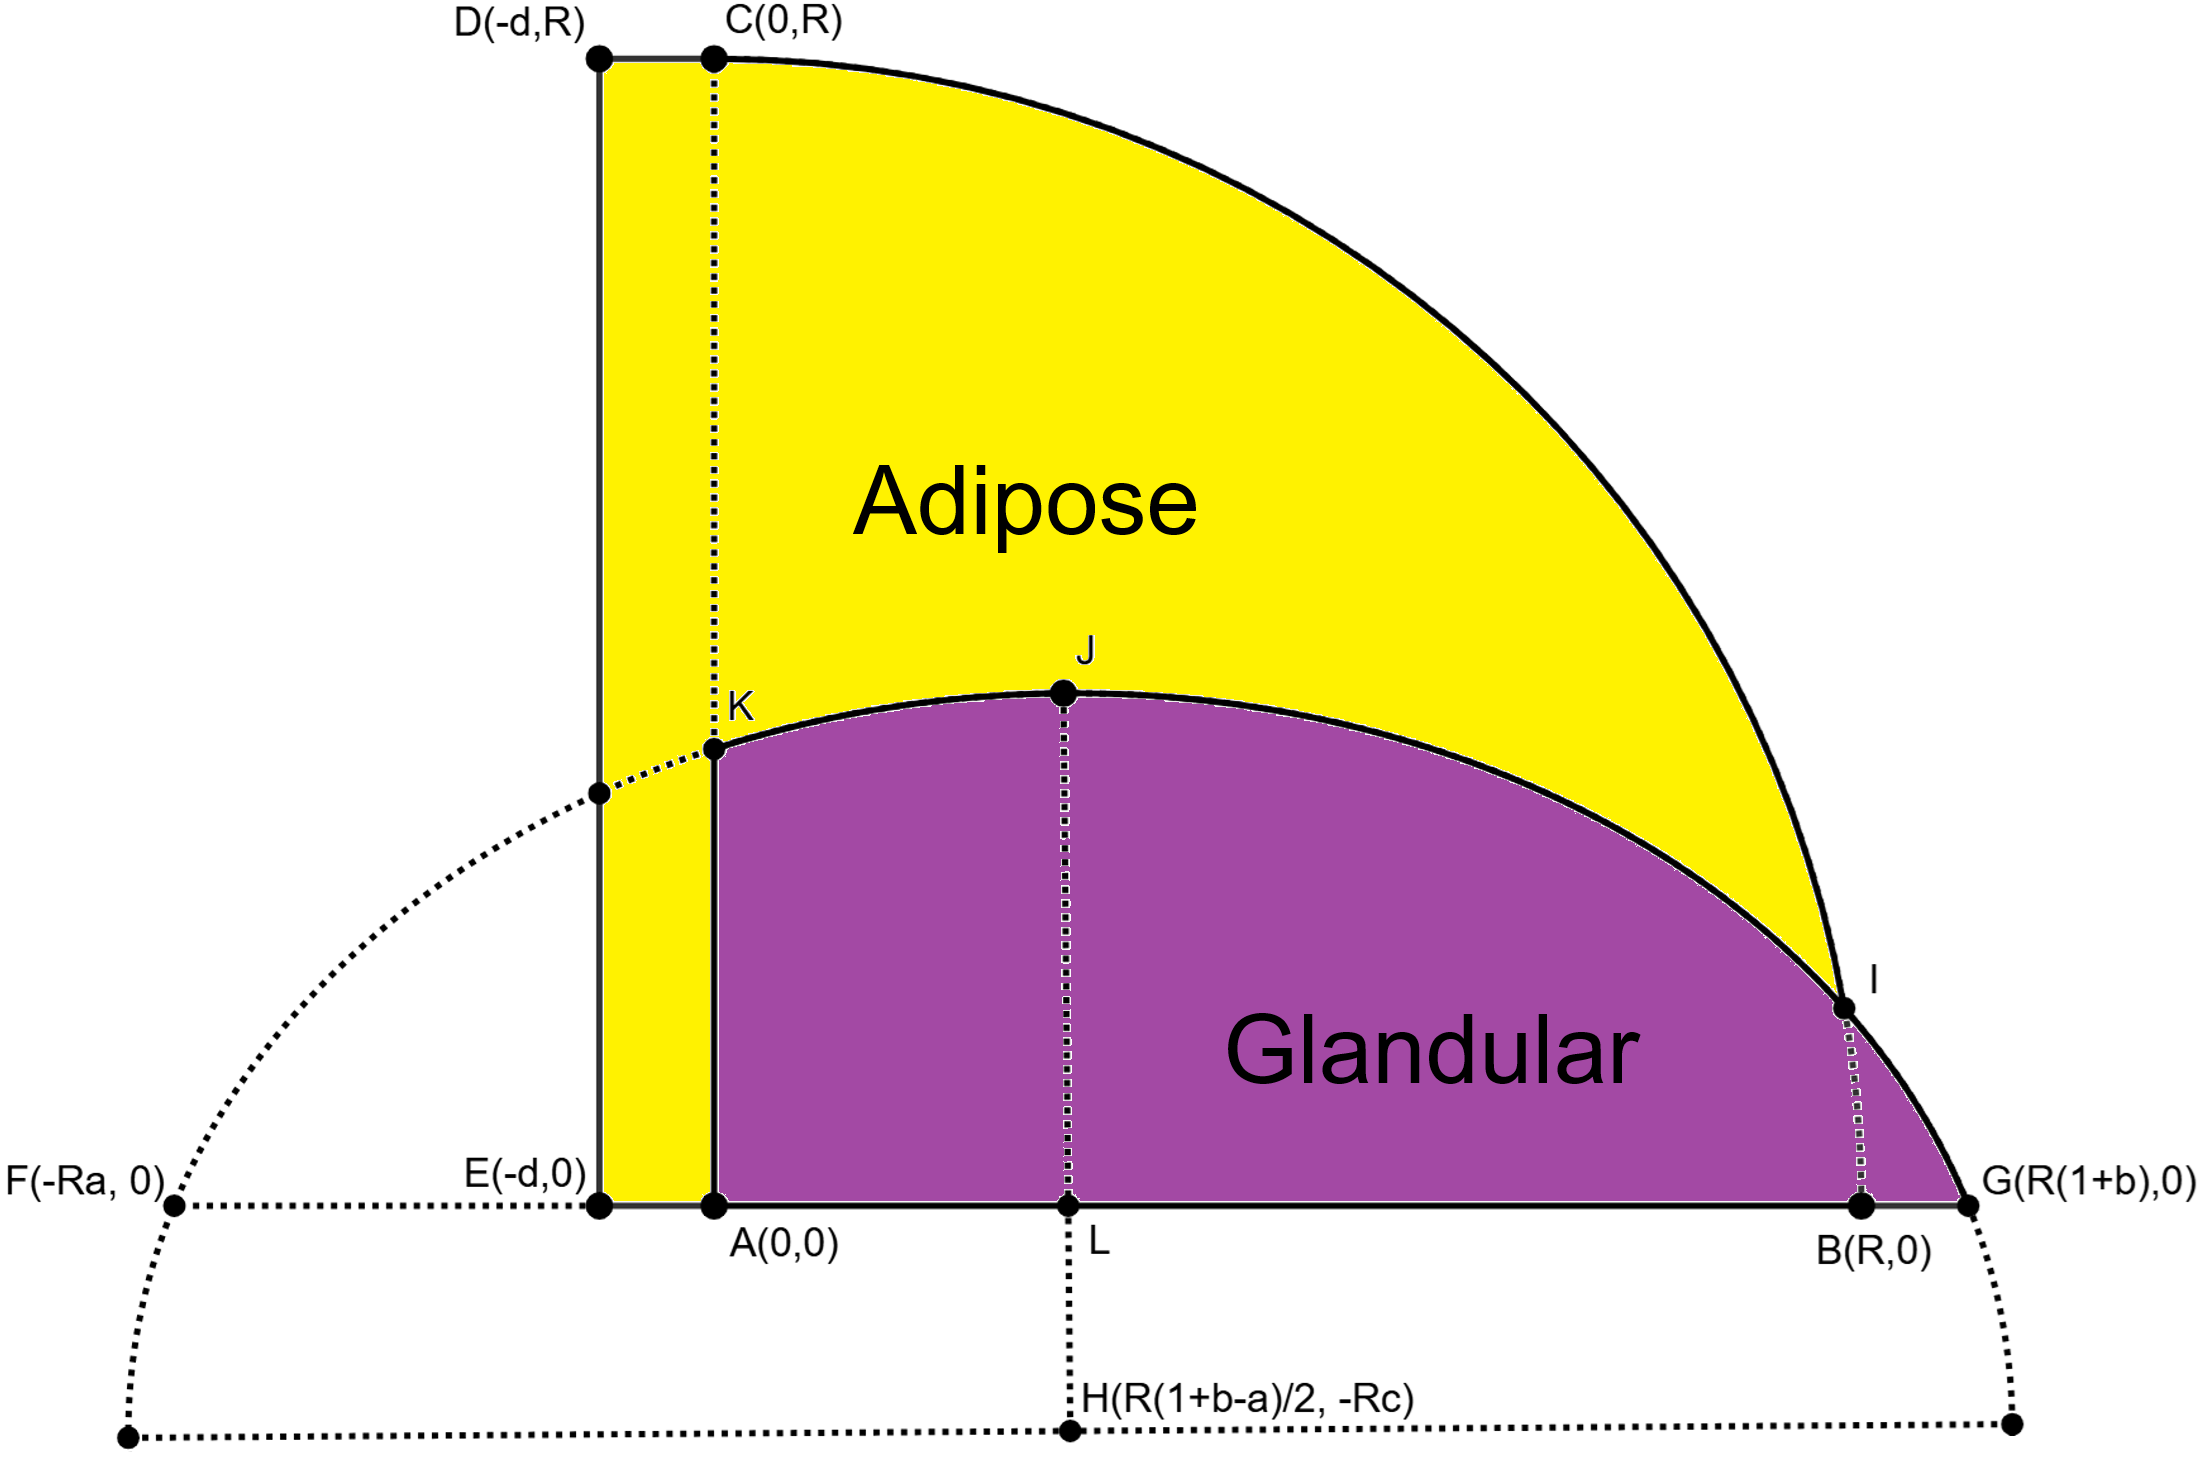
\includegraphics[width=0.85\linewidth]{Figures/Appendix/breast_crossesction.png}
\caption{Schematic cross-section from the earlier EWS FEM breast model by R. Engels \cite{EngelsEWSReport}. The figure illustrates the parametrised adipose and glandular regions used in that previous modelling route and is included here as internal methodological context.}
\label{fig:appendix_previous_ews_cross_section}
\end{figure}

The later EWS/SIOUX workflow provided additional context for skin representation, soft material settings and distributed reinforcement concepts for Cooper-ligament-like support \cite{StormEWSReport}. In the current project, these earlier modelling choices were treated as reference points rather than as fixed requirements. The COMSOL route was developed as a separate implementation with emphasis on controlled geometry construction, automated region definitions, build-only checks and systematic comparison between model variants. This made it possible to investigate selected anatomical and mechanical modelling assumptions in a more traceable way, without implying that the current model is a validated patient-specific representation.

\newpage
\section{Current COMSOL repository and reproducibility structure}
\label{sec:appendix_current_repository}

The active implementation used in this internship project is the COMSOL source-case pipeline developed during this project. The public project repository stores the reproducible parts of the work, including the Python source code, active TOML case definitions, report notes, plotting scripts, compact post-processing tables and selected figures \cite{KuijpersEWSComsolGitHub}. Large generated COMSOL files, build folders, solve folders, recovery files and raw exports are not intended to be stored in the repository because they can become several gigabytes per case.

The main repository folders used for the current COMSOL workflow are summarised in Table~\ref{tab:appendix_repository_structure}. The exact folder structure may still change during repository cleanup, but the distinction between source definitions, generated artefacts and compact evaluation output was maintained throughout the project.

\begin{table}[H]
\centering
\caption{Main repository components used in the COMSOL model-development workflow.}
\label{tab:appendix_repository_structure}
\begin{tabular}{p{0.40\linewidth} p{0.50\linewidth}}
\toprule
Repository component & Role in the project \\
\midrule
\texttt{src/ews\_fem\_pipeline\_comsol} & Active Python package for the COMSOL source-case workflow, including case loading, model generation support, Java builder generation, run control and post-processing utilities. \\
\texttt{runs/comsol\_runs} & Version-controlled TOML case definitions for the main model variants and sensitivity studies. \\
\texttt{analysis\_output/comsol\_pipeline} & Compact evaluation outputs used for comparison, including summary tables, selected plots and post-processing results. \\
\texttt{docs/report\_notes/comsol\_pipeline} & Project notes documenting modelling choices, run status, figure sources and interpretation decisions. \\
\texttt{docs/Internship\_report\_Daan\_Kuijpers} & The final intership project report. \\
\bottomrule
\end{tabular}
\end{table}

The COMSOL simulations were run using a licensed COMSOL Multiphysics installation available through TU/e. Most model builds and dynamic solves were executed on local hardware during model development. Because time-dependent COMSOL solves can be computationally expensive, especially for second-order elements, volumetric skin layers and larger parameter sweeps, access to stronger computational resources such as TU/e high-performance computing facilities is relevant for future large-scale studies. In this project, the repository was therefore organised to preserve the reproducible case definitions and compact outputs, while allowing heavy generated artefacts to remain outside version control.

\newpage
\section{Simplified example of a COMSOL case definition}
\label{sec:appendix_example_case_definition}

The COMSOL pipeline uses TOML case definitions to specify the main model settings. The full case files contain more detailed options than shown below. Listing~\ref{lst:appendix_simplified_toml} gives a simplified example to illustrate how geometry, material, loading and evaluation settings are defined in a traceable format.

\begin{lstlisting}[
caption={Simplified example of a COMSOL case definition. Only the main settings are shown; the complete case definitions are stored in the project repository.},
label={lst:appendix_simplified_toml}
]
[case]
name = "example_reference_case"
description = "Simplified reference case for documentation"

[geometry]
breast_volume_ml = 585
chestwall_variant = "xoffset055"
glandular_distribution = "realistic_reference"
outer_shape_asymmetry = "none"

[materials]
adipose_set = "reference"
glandular_set = "reference"
skin_layer = "none"
cooper_support = "none"

[loading]
type = "fixed_support_acceleration"
amplitude_g = 0.25
duration_s = 0.60
mass_damping_alpha = 60

[tumor]
enabled = false

[evaluation]
export_displacement = true
export_von_mises_stress = true
export_surface_metrics = true
\end{lstlisting}

The purpose of these case definitions is not only to automate COMSOL runs, but also to make the modelling assumptions explicit. When a model variant is changed, the corresponding TOML file records which geometry, material, loading or evaluation setting was modified. This makes comparisons between model variants more transparent than manually editing a single COMSOL model file for each simulation.

\newpage
\section{Breast-volume reference data}
\label{sec:appendix_breast_volume_reference}

An internal Catharina Hospital breast-volume dataset was reviewed to contextualise the selected COMSOL reference volume. The dataset consisted of 100 manually delineated breast volumes. The contours were drawn approximately 5~mm inside the outer skin boundary on images acquired in a supine position. The reported values should therefore be interpreted as internal reference volumes for model scaling, rather than as exact external breast volumes.

\begin{table}[H]
\centering
\caption{Summary of the internal Catharina Hospital breast-volume reference dataset. The dataset contained 100 manually delineated breast volumes, with contours drawn approximately 5~mm inside the outer skin boundary in supine images.}
\label{tab:appendix_breast_volume_reference}
\begin{tabular}{lc}
\toprule
Metric & Breast volume (mL) \\
\midrule
Mean & 728.32 \\
Median & 691.15 \\
Standard deviation & 327.39 \\
25th percentile & 519.65 \\
75th percentile & 928.70 \\
Minimum & 105.68 \\
Maximum & 1777.28 \\
\bottomrule
\end{tabular}
\end{table}

The selected COMSOL reference volume of $\sim$585~mL lies between the 25th percentile and the median of this internal dataset. This supports its use as a lower-mid reference volume for the current model-development route. Direct comparison remains limited by the segmentation definition and patient position, because the internal contours were drawn inside the skin boundary and in a supine position.

The internal dataset was also compared with literature values for breast-volume measurement. Stahl et al. reported MRI-based breast anthropometry in a cohort of 400 women and showed a broad distribution of breast volumes \cite{Stahl2023}. Yoo et al. compared MRI-estimated breast volume with mastectomy specimen weight and supports the clinical relevance of MRI-based volume estimation, although in a cancer/mastectomy cohort \cite{Yoo2013}. Nie et al. showed that skin removal can change quantitative MRI-based breast-volume and density measurements, which is relevant because the internal dataset was delineated inside the outer skin boundary \cite{Nie2010SkinRemoval}. Choppin et al. reviewed breast-volume measurement methods and emphasised that measurement uncertainty depends strongly on method, patient pose and boundary definition \cite{Choppin2016}. Together, these sources support using the $\sim$585~mL COMSOL volume as a defensible controlled reference volume, while avoiding overinterpretation as an exact population average.

\newpage
\section{Fibroglandular fraction reference data}
\label{sec:appendix_glandular_fraction_reference}

The selected Stage~3 reference model was compared with literature on volumetric breast density and fibroglandular tissue quantification. This comparison was used to contextualise the chosen fibroglandular fraction, not to assign a clinical BI-RADS category to the model.

\begin{table}[H]
\centering
\caption{Literature context used to interpret the selected fibroglandular fraction. The model fraction refers to three-dimensional fibroglandular volume divided by total breast volume.}
\label{tab:appendix_glandular_fraction_reference}
\begin{tabular}{p{0.30\linewidth} p{0.58\linewidth}}
\toprule
Source & Relevance for this model \\
\midrule
Sartor et al. \cite{Sartor2016} & Compares qualitative radiologist density classification with automated volumetric assessment and provides context for volumetric density groups. \\
Nie et al. \cite{Nie2010} & Quantifies three-dimensional fibroglandular tissue patterns from MRI and reports volumetric breast and fibroglandular tissue measurements. \\
Lu et al. \cite{Lu2012} & Compares breast tissue measurements across MRI, mammography and mathematical estimation, and shows that individual fibroglandular fractions can vary substantially. \\
ACR BI-RADS \cite{ACRBIRADS} & Provides the clinical breast-composition framework, but these categories are not directly equivalent to the model's three-dimensional fibroglandular volume fraction. \\
\bottomrule
\end{tabular}
\end{table}

This density context is also relevant for the EWS application. Women with dense breasts are more difficult to screen using X-ray mammography because fibroglandular tissue can reduce lesion conspicuity and lower mammographic sensitivity \cite{VonEuler-Chelpin2019,Bakker2019}. For this reason, a relatively fibroglandular-rich reference model is useful for EWS-oriented model development, provided that it is not interpreted as a population-average breast composition.

The selected COMSOL reference case produced a breast volume of approximately 585~mL and a glandular fraction of 24.308\%, corresponding to an approximate glandular volume of 142.2~mL. This value is higher than typical average volumetric density values reported in screening populations, but remains defensible as a controlled fibroglandular-rich reference for EWS-oriented model development. It should therefore be interpreted as a selected anatomical reference configuration rather than as a population-average breast-density value or a direct BI-RADS category.

\newpage
\section{Material-parameter literature summary}
\label{appendix_material_parameter_literature_summary}

The material parameters used in the COMSOL model were selected as controlled reference and sensitivity values rather than as patient-specific tissue measurements. Reported breast-tissue stiffness values vary strongly between studies because they depend on measurement protocol, tissue preparation, preload, strain level, loading direction, subject characteristics and constitutive model \cite{Samani2007,Ramiao2016,Goodbrake2022,Teixeira2023}. The literature was therefore used to define plausible stiffness scales and sensitivity ranges, not to identify one unique material parameter set.

\begin{table}[H]
\centering
\small
\caption{Summary of the literature-based rationale used for selecting the material-parameter scales in the COMSOL model.}
\label{appendix_material_parameter_rationale_table}
\begin{tabular}{p{0.20\linewidth} p{0.34\linewidth} p{0.36\linewidth}}
\toprule
Model component & Literature interpretation & Use in the COMSOL model \\
\midrule
Adipose tissue 
& Normal breast adipose tissue is generally reported in the low-kPa stiffness range, although values differ between ex-vivo testing, elastography and model calibration studies \cite{Samani2007,Ramiao2016,Teixeira2023}. 
& The reference adipose material was assigned an approximate small-strain stiffness of $E\approx3.66~\mathrm{kPa}$. Softer and intermediate variants were included as material-stiffness sensitivity cases. \\

Fibroglandular tissue 
& Fibroglandular tissue is typically stiffer and more heterogeneous than adipose tissue. Three-dimensional testing also indicates that human breast tissue can show direction-dependent and spatially heterogeneous behaviour \cite{Goodbrake2022}. 
& The reference fibroglandular material was assigned an approximate small-strain stiffness of $E\approx10~\mathrm{kPa}$. Additional variants were used to test the sensitivity of the simulated response to internal tissue stiffness. \\

Skin layer 
& Skin is mechanically relevant in breast deformation models and is commonly represented as a stiffer component than the internal breast tissues. Its effective contribution depends on both material stiffness and layer thickness \cite{Chen2025,Teixeira2023}. 
& The active volumetric-skin route used a thickness of $1.5~\mathrm{mm}$ and an approximate stiffness scale of $E\approx500~\mathrm{kPa}$. Lower skin-stiffness cases were retained only as sensitivity variants. \\

Tumor overlay 
& Tumor tissue is generally reported to be stiffer than surrounding normal tissue, but the reported stiffness range depends strongly on imaging modality, tissue type and region of interest \cite{Samani2007,McKnight2002,Patel2021,Patel2022}. 
& The hard tumor-overlay setting targeted an approximate stiffness scale of $E\approx100~\mathrm{kPa}$. This value was used to create a clear stiffness contrast, not as a patient-specific tumor calibration. \\

Posterior support 
& The posterior thoracic region was not modelled as a detailed anatomical chest wall. Instead, it was included as a simplified mechanical support region for the breast model. 
& The constructed posterior support domain was assigned a linear elastic surrogate material with $E=10~\mathrm{kPa}$ and $\nu=0.49$. \\
\bottomrule
\end{tabular}
\end{table}

Overall, the selected parameters should be interpreted as a controlled modelling set for comparing material routes and sensitivity cases. The values define consistent stiffness scales for the COMSOL workflow, while acknowledging that breast tissue, skin and tumor properties cannot be represented by a single universally accepted parameter value.





%%%%%%%%%%%%%%%%%%%%%%%%%%%%% eruit of veranderen appendix hieronder
\newpage
\section{Figure and metric sources}
\label{sec:appendix_figure_metric_sources}

The figures and quantitative values in the main report are based on selected COMSOL outputs, compact post-processing files and generated plots. The complete figure and metric source index is stored in \texttt{docs/report\_notes/comsol\_pipeline/report\_figures\_metrics\_index.md}. This index records the relevant COMSOL output folders, metric files and source images used to create the report figures.

The appendix figures below are included as provenance material. They document the source contact sheets and geometry screenshots used during model development. They are not all intended to carry the same quantitative interpretation as the main results.

\begin{figure}[H]
\centering
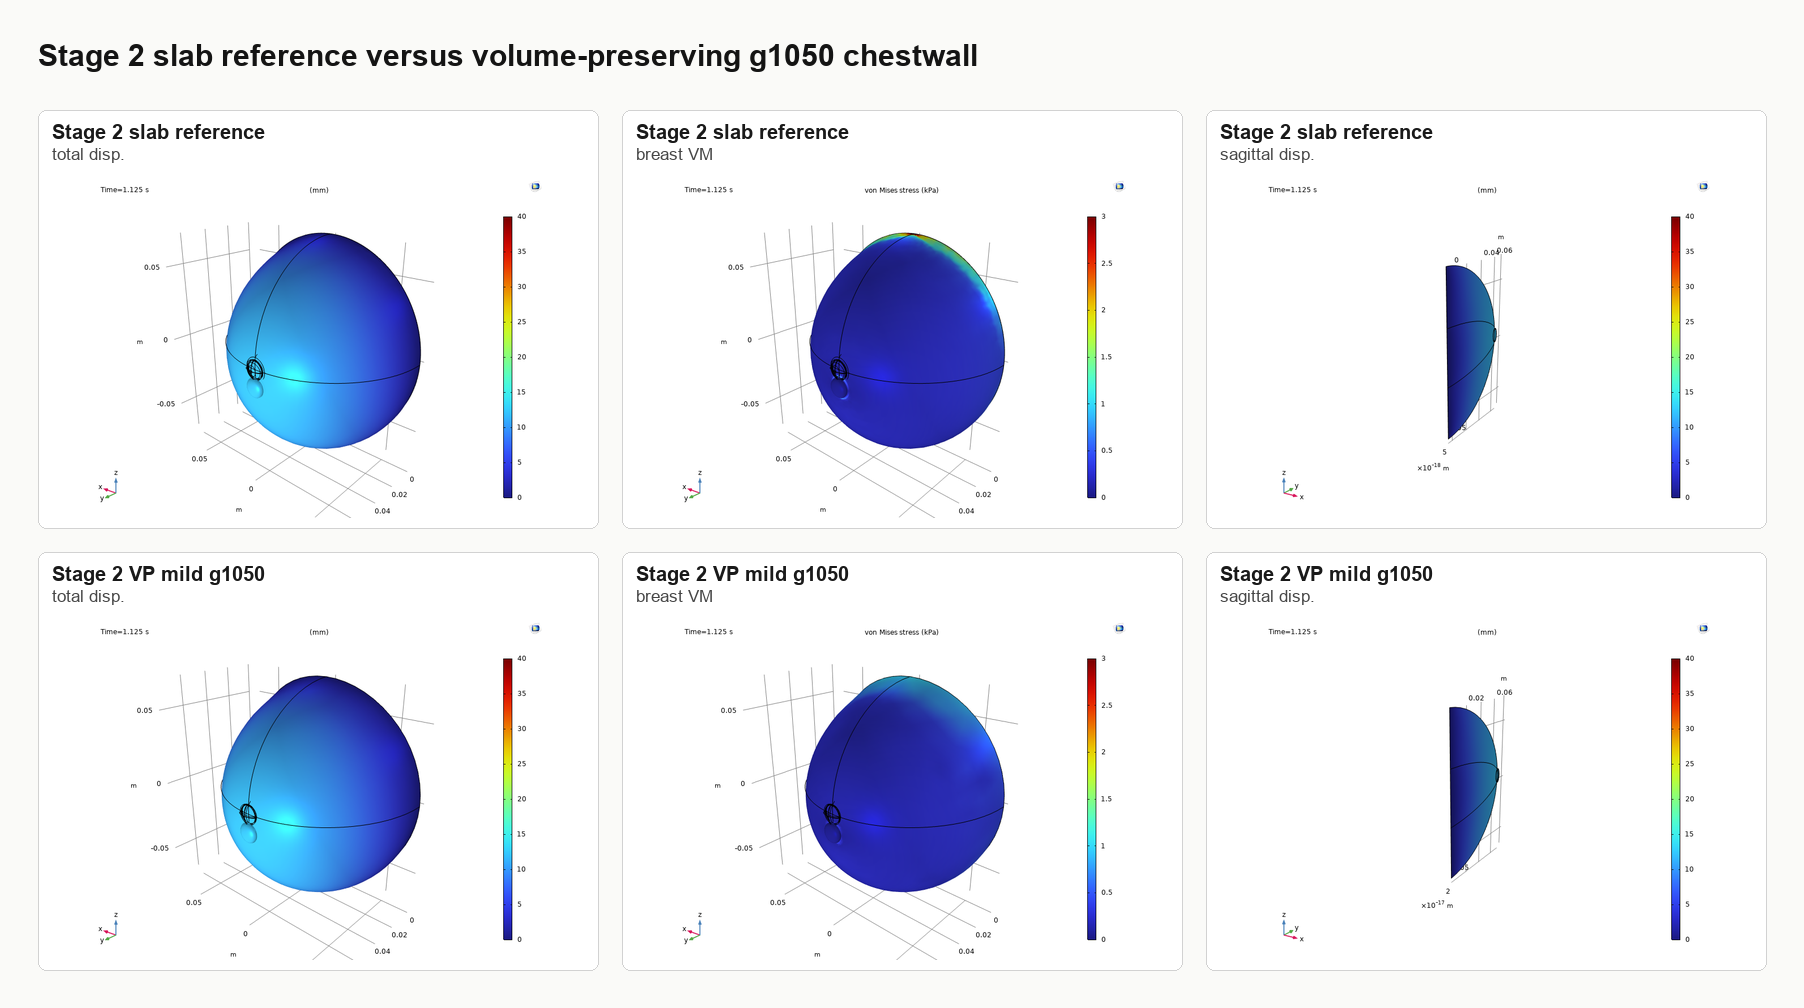
\includegraphics[width=0.95\linewidth,height=0.78\textheight,keepaspectratio]{Figures/comsol_contact_sheets/stage2_chestwall_contact_sheet.png}
\caption{Source contact sheet for the selected chestwall-geometry route. The figure documents displacement and von Mises stress panels used during the evaluation of the curved posterior support geometry.}
\label{fig:appendix_stage2_figures}
\end{figure}

\begin{figure}[H]
\centering
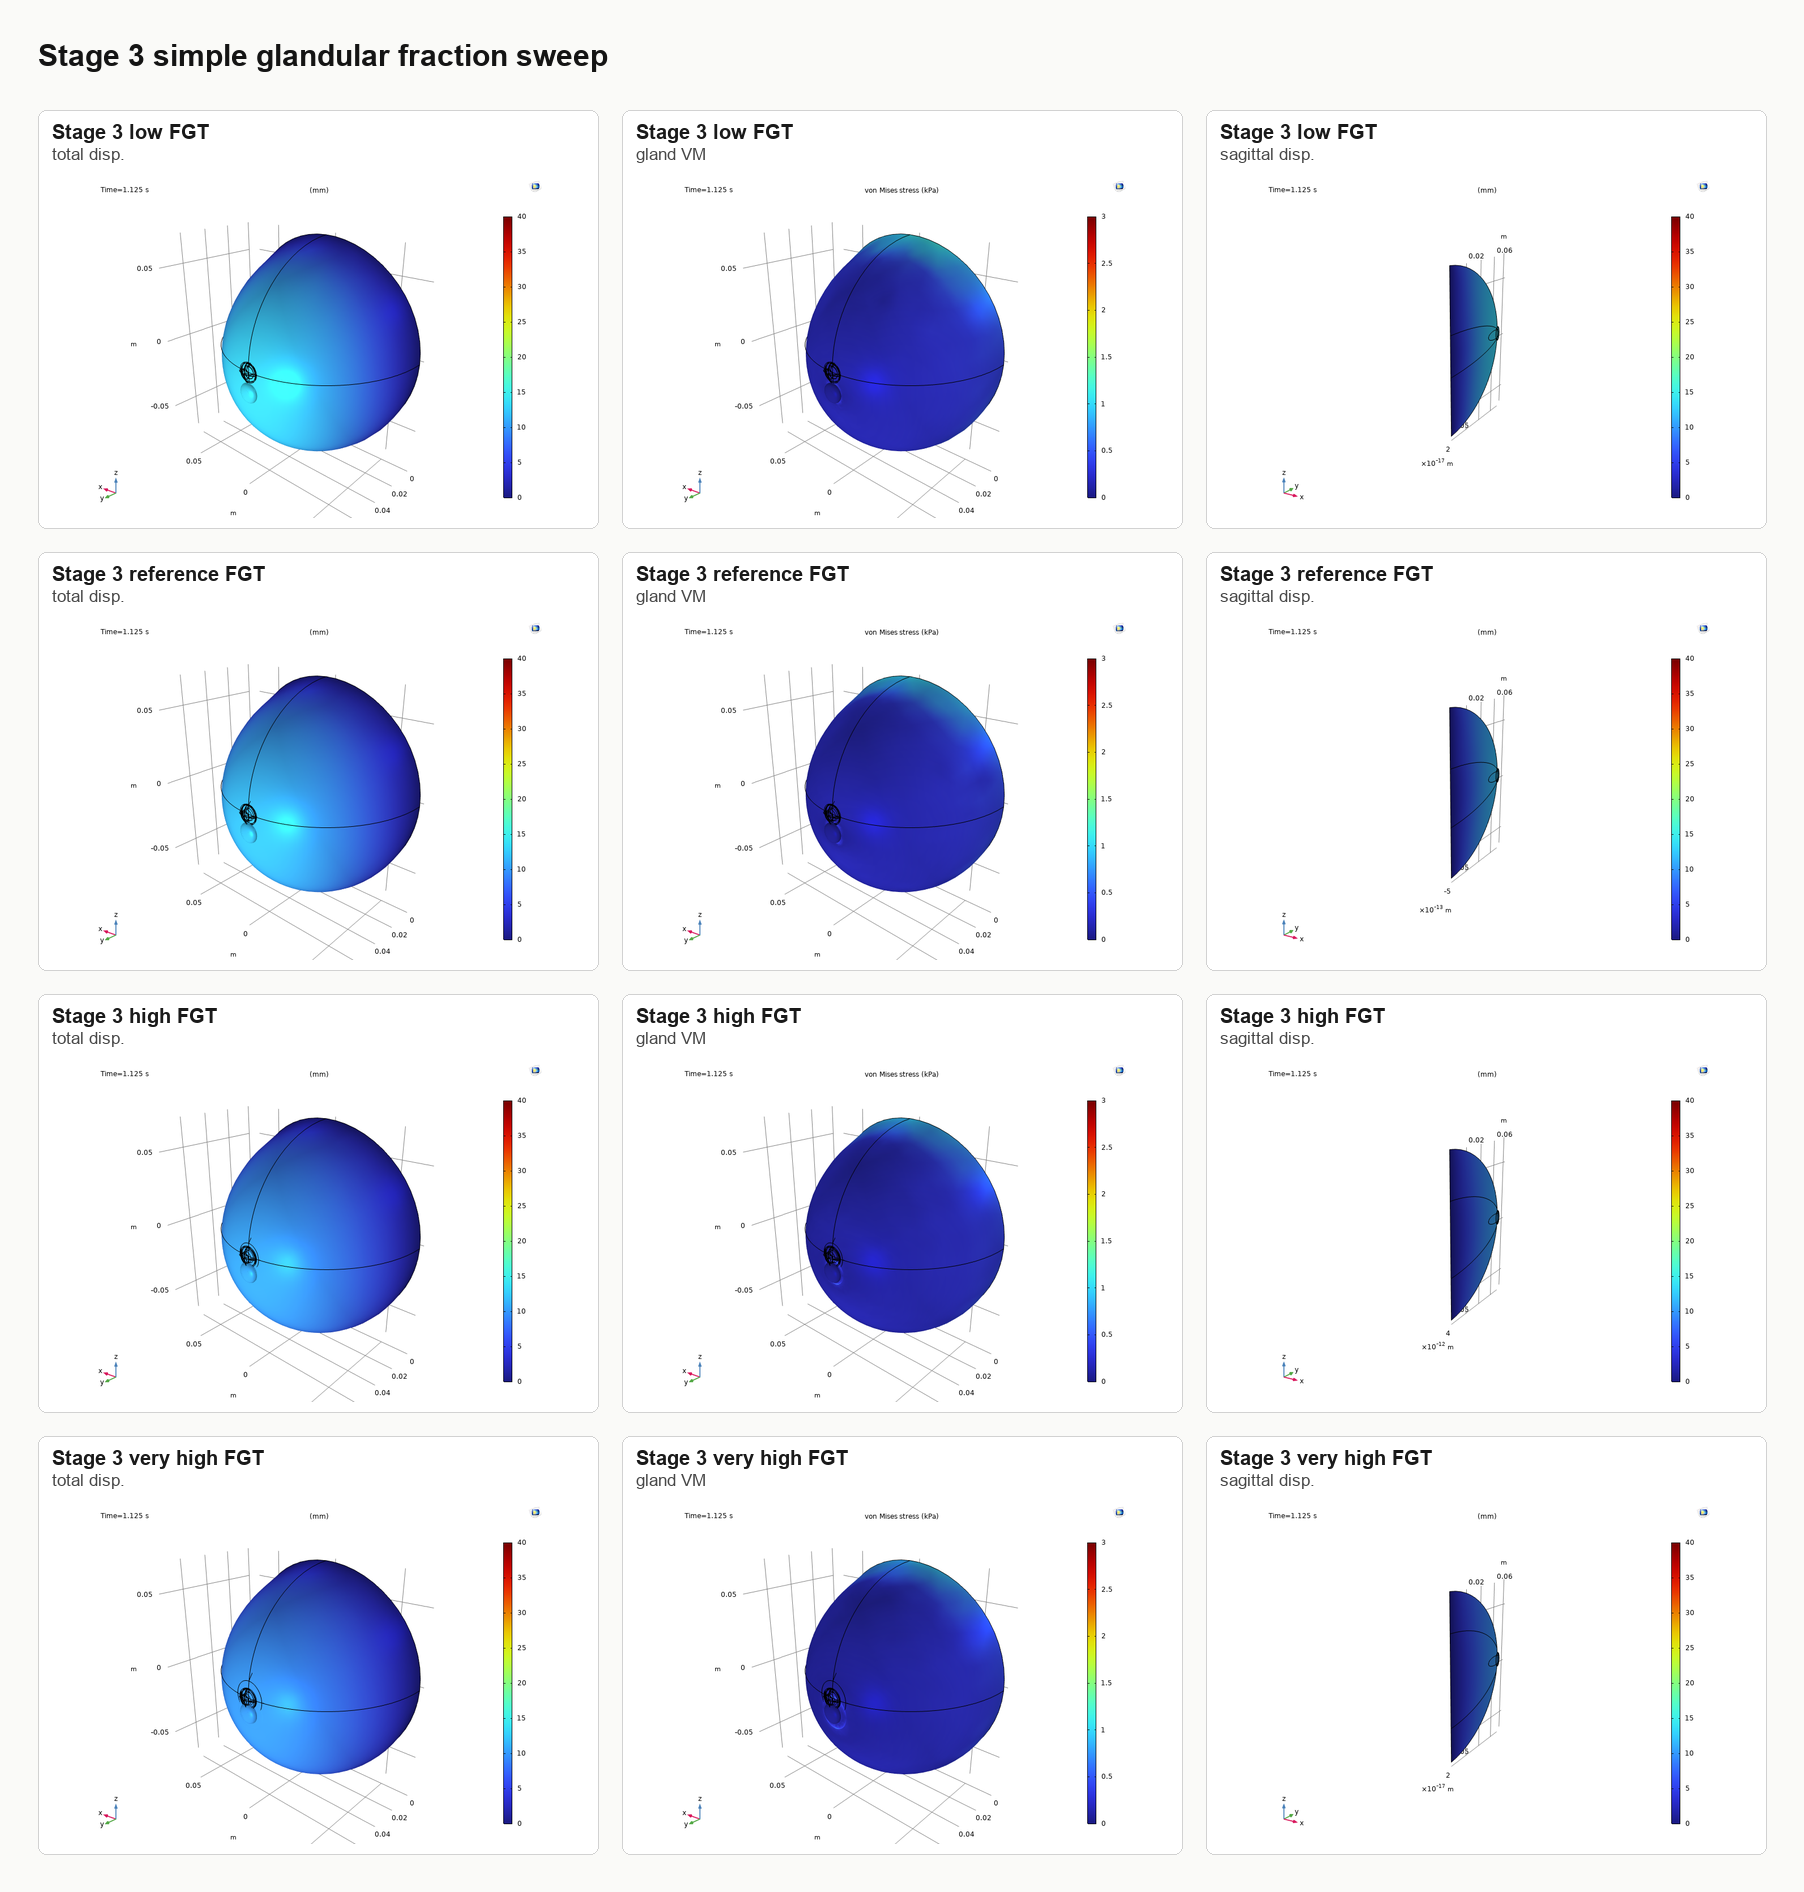
\includegraphics[width=0.95\linewidth,height=0.78\textheight,keepaspectratio]{Figures/comsol_contact_sheets/stage3_glandular_fraction_contact_sheet.png}
\caption{Source contact sheet for the glandular-distribution comparison. The figure documents the solved simple glandular fraction sensitivity and supports the transition toward a more realistic glandular reference.}
\label{fig:appendix_stage3_fraction_figures}
\end{figure}

\begin{figure}[H]
\centering
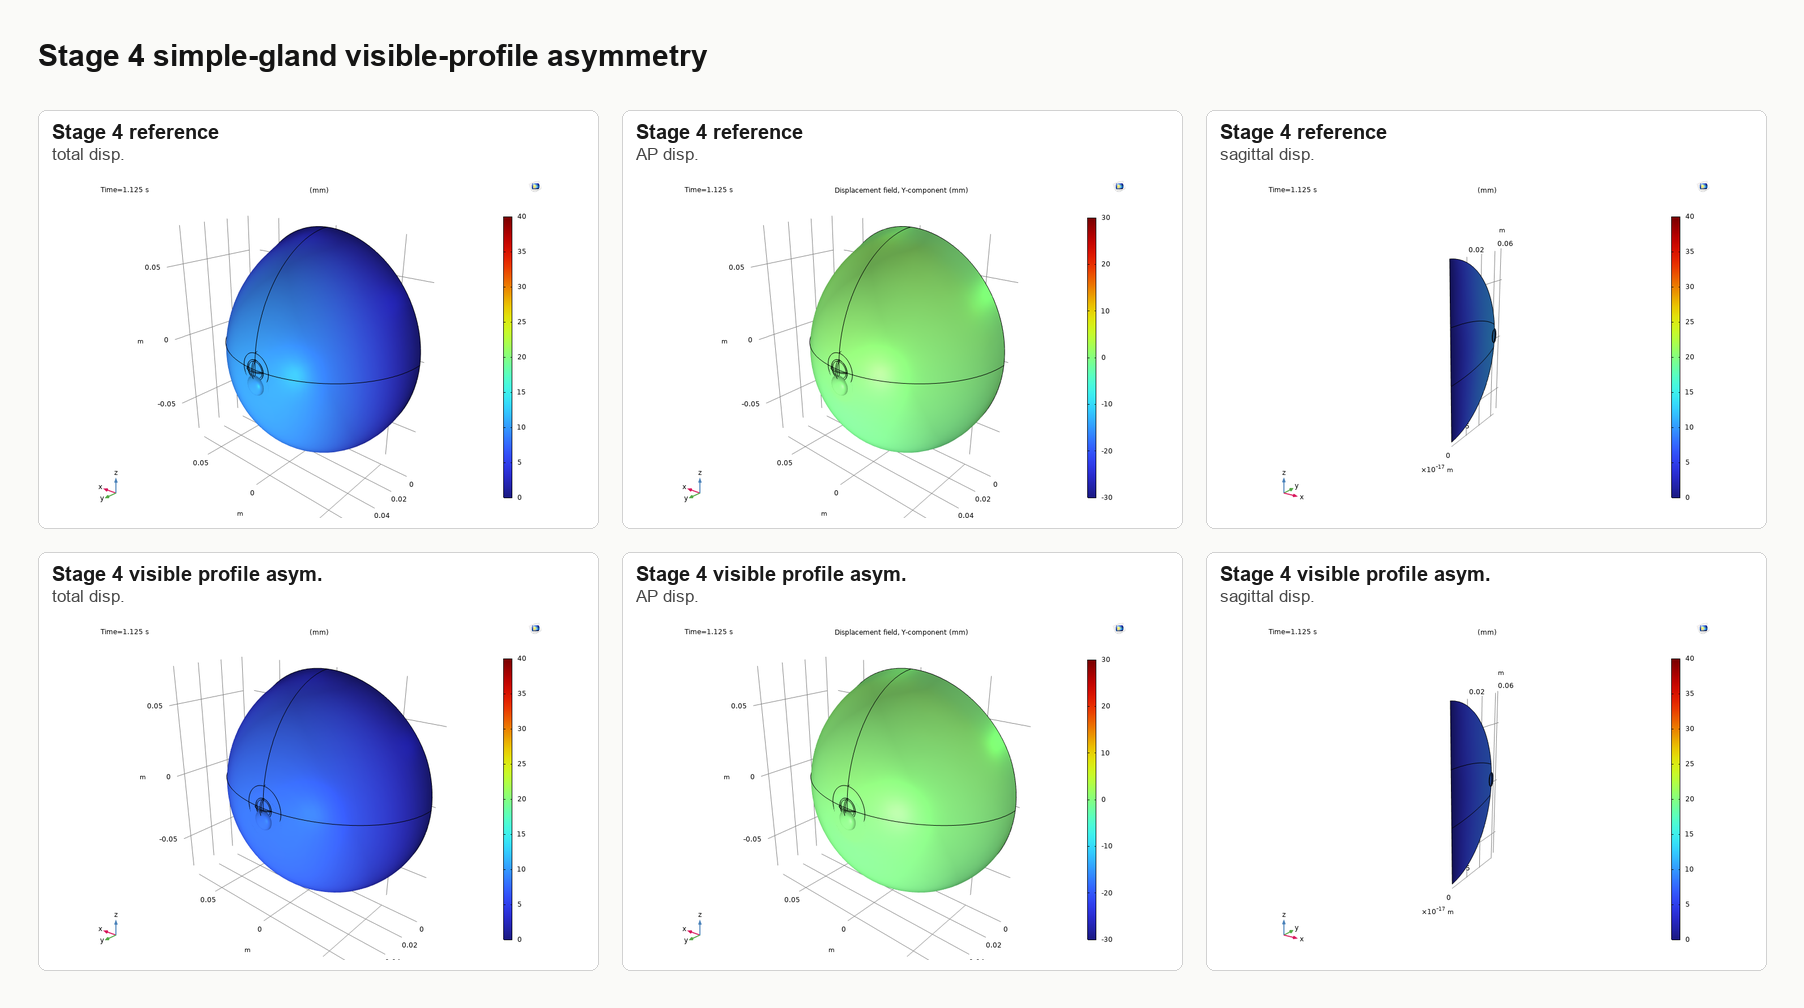
\includegraphics[width=0.95\linewidth,height=0.78\textheight,keepaspectratio]{Figures/comsol_contact_sheets/stage4_asymmetry_contact_sheet.png}
\caption{Source contact sheet for outer-shape and nipple-position sensitivity checks. These cases are used as geometry-development context and should be interpreted separately from the matched reference comparisons.}
\label{fig:appendix_stage4_figures}
\end{figure}

\begin{figure}[H]
\centering
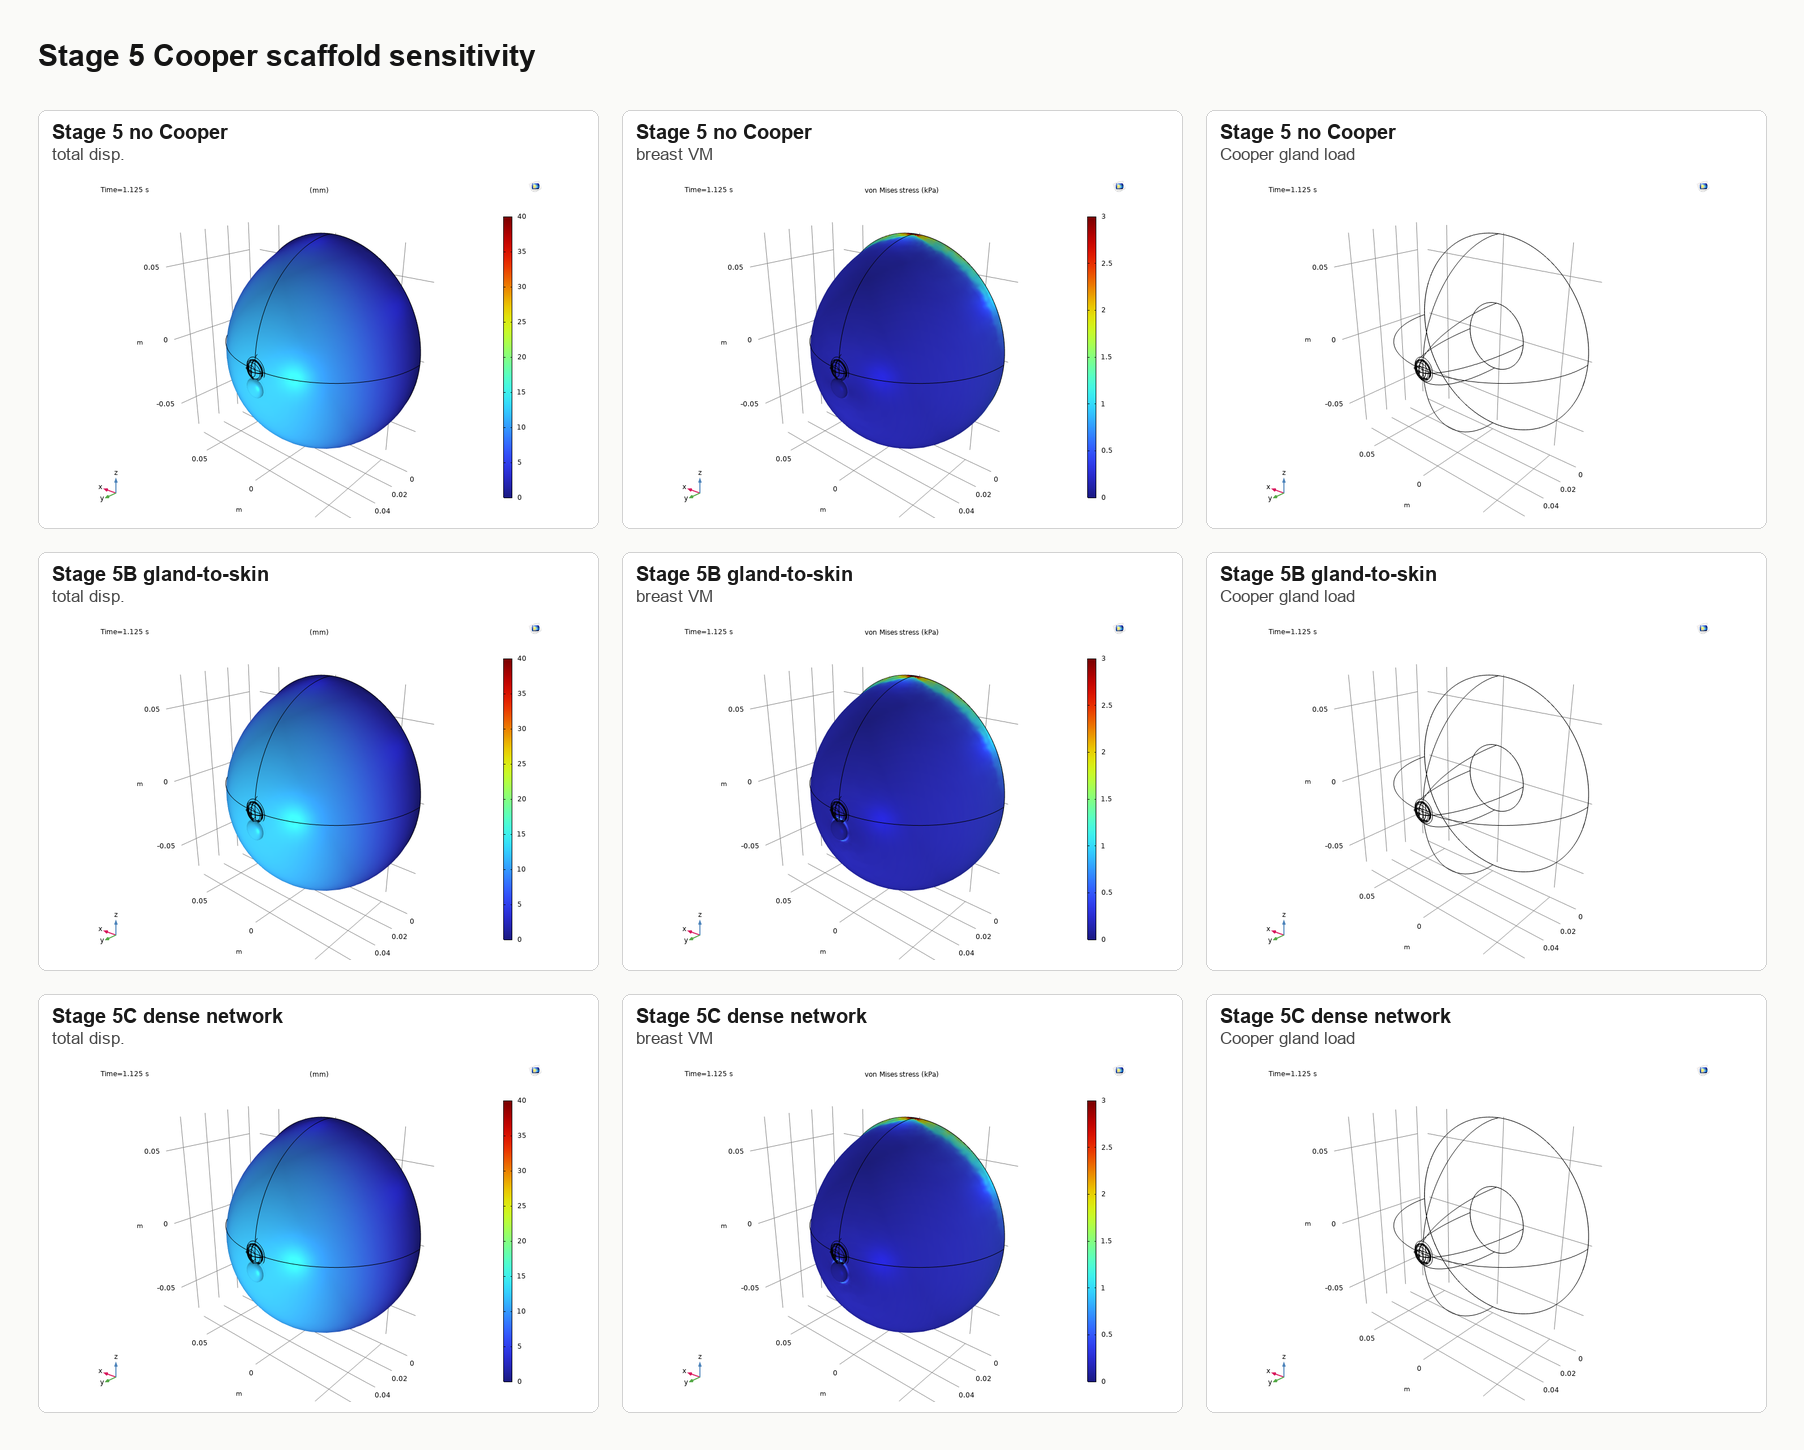
\includegraphics[width=0.95\linewidth,height=0.78\textheight,keepaspectratio]{Figures/comsol_contact_sheets/stage5_cooper_contact_sheet.png}
\caption{Source contact sheet for the Cooper-support development branch. The stable reference interpretation uses the no-Cooper control unless a Cooper-support variant solves robustly and produces complete post-processing output.}
\label{fig:appendix_stage5_figures}
\end{figure}
